% background chapter continued

%\section{Consistent Hashing}\index{Consistent Hashing}

\pagebreak

\section{Event-Driven Architecture}\label{eventdriven}
This style is different from traditional request/response programming model where the interaction
between different components are accomplished by announcing events that have already occurred. An
event does not hold any logic but contains a piece of data describing something has happened inside the
application. Being able to identify parts of the application that fit into this model can positively
impact on scalability.

\subsection{Message Queues (MQ)}
MQs are one such tool for achieving asynchronous behavior in the application even if the programming
language in use does not support it.

\begin{figure}[h!]
  \centering
  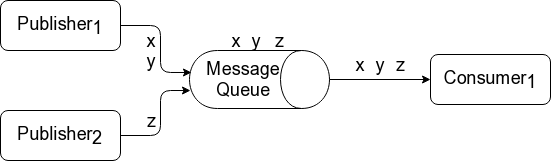
\includegraphics[width=10cm,height=6cm,keepaspectratio]{../media/crawler/mq_basic.png}
  \caption{Message Queue with Producers and Consumers}
  \label{fig:mqbasics}
\end{figure}

\noindent
MQ buffers messages and distributes it in asynchronous fashion. A message is XML/JSON data containing
all information required to perform an operation. Requests served through MQs are always unidirectional,
one-way, fire-and-forget style. Figure \ref{fig:mqbasics} shows MQ involves a producer/publisher on one
side and consumer on other side. Producers push message to the queue which is buffered and finally
delivered to active consumer.
\begin{description}
  \item[decoupling] \hfill \\
    message queues deliver the highest degree of decoupling. The biggest one is different language
    runtime.
  \item[scaled independently] \hfill \\
    Producer and consumers can be horizontal scaled separately without overloading the system. The processes
    can also be hosted on completely separate machines.
  \item[balancing traffic] \hfill \\  
    Immediate advantage after scaling to separate machines is evening out spikes in capacity handling. This
    increases availability because messages produced are enqueued quickly before consumer can process it at
    its capacity.
  \item[fault-tolerance] \hfill \\
    publishers and consumers are not affected by each others failure instances as they are not directly
    bound to each other but through intermediary such as queue, therefore, message processing can be
    stopped at any time for maintenance. Similarly, a hardware failure can be replaced with new machine
    without bringing the entire application to halt.

    \pagebreak

  \item[async processing] \hfill \\
    Producers and consumer work independently and constraint only by adhering to request format. This
    separation between producer and consumer enables non-blocking, asynchronous processing. Neither of them
    wait for each other to become available.
\end{description}

\subsection{RabbitMQ as a Message Broker}
A message queue\cite{asyncmsg} can simply be seen as utility powered with SQL database. But there exist dedicated message
broker which houses essential functionality such as message routing and delivery, permission control, and
failure recovery. All this makes working with them easy. Brokers are sophisticated implementation of
message queues. They are also called "message-oriented middleware".
\begin{figure}[h!]
  \centering
  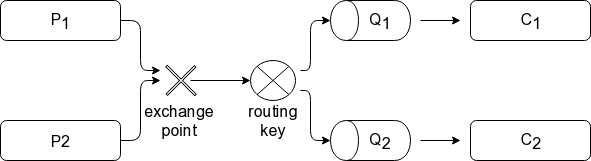
\includegraphics[width=14cm,height=10cm,keepaspectratio]{../media/crawler/rmq_exchange.png}
  \caption{RabbitMQ broker terminology}
  \label{fig:mqexchange}
\end{figure}

\noindent
RabbitMQ\cite{asyncmsg} is a high-performance, generic message passing platform. This broker uses configuration over code
to perform request routing and delivery. It exposes an API to dynamically configure routing. It speaks
AMQP, STOMP messaging protocols, various client libraries exist to communicate with rabbitmq. The
separation between publishers and consumers is accomplished through a concept called as exchange points as
shown in figure \ref{fig:mqexchange}. Producers $P_1$, $P_2$ has to known the name of the exchange only to
enqueue the message in the right queue which is later consumed by consumer $C_1$, $C_2$. Moreover, RabbitMQ
also supports complex routing through custom routing key patterns, along with built-in patterns like
direct worker queue and pub/sub.